\documentclass{prova}

\usepackage{amsmath}
\usepackage{amsfonts}

\setlength{\textheight}{25cm}

\DeclareMathOperator{\sen}{sen}
\DeclareMathOperator{\tg}{tg}
\newcommand{\ds}{\displaystyle}

\professor{Prof.\@ Adriano Barbosa}
\disciplina{C\'alculo Diferencial e Integral}
\avaliacao{P2}
\curso{Engenharia de Computa\c{c}\~ao}
\data{06/06/2022}

\begin{document}
	\cabecalho{5}  % o numero 5 indica a qnt de quadros na tabela de nota

    \textbf{Todas as respostas devem ser justificadas.}

    \begin{questionario}
        \q{Calcule o limite $\displaystyle\lim_{x\rightarrow 1^{+}}
           x^{\frac{1}{1-x}}$.}

        \q{Cada lado de um quadrado est\'a aumentando a uma taxa de 3cm/s. A que
           taxa a \'area do quadrado est\'a aumentando quando sua \'area \'e 12cm$^2$?}

        \q{Explique o efeito de cada linha abaixo no gr\'afico de $f$ e esboce o
           gr\'afico da fun\c{c}\~ao tal que:}

            $f(0)=0, f'(-2)=f'(1)=f'(9)=0$ \\
            $\displaystyle\lim_{x\rightarrow\infty} f(x)=0, \lim_{x\rightarrow
            6} f(x)=-\infty$ \\
            $f'(x)<0$ em $(-\infty,-2), (1,6)$ e $(9,+\infty)$ \\
            $f'(x)>0$ em $(-2,1)$ e $(6,9)$ \\
            $f''(x)>0$ em $(-\infty,0)$ e $(12,+\infty)$ \\
            $f''(x)<0$ em $(0,6)$ e $(6,12)$

        \q{Calcule a \'area entre as curvas $y=-x^2+3x$ e $y=x$.}
            \begin{figure}[h]
                \centering
                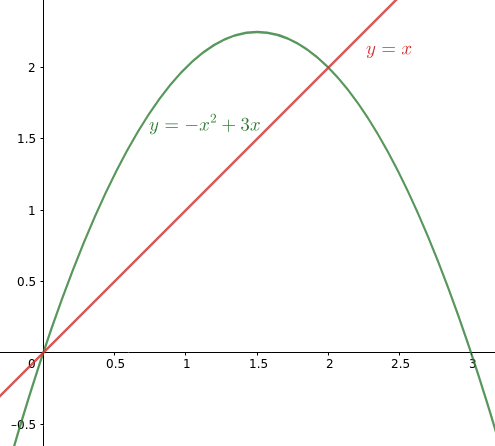
\includegraphics[width=0.4\textwidth]{fig1.png}
            \end{figure}

        \q{Calcule o volume da regi\~ao delimitada por $x=1+y^2$, $y=x-3$
           rotacionada ao redor do eixo $y$.}
    \end{questionario}
\end{document}
